% !TeX program = xelatex
\documentclass{assignment}
\usepackage[UTF8,scheme=chinese,fontset=none]{ctex}
\setCJKmainfont[Path=../assets/fonts/,BoldFont=FandolSong-Bold.otf,ItalicFont=FandolKai-Regular.otf]{FandolSong-Regular.otf}
\setCJKsansfont[Path=../assets/fonts/,BoldFont=FandolHei-Bold.otf]{FandolHei-Regular.otf}
\setCJKmonofont[Path=../assets/fonts/]{FandolHei-Regular.otf}
\usepackage{cite}
\usepackage{tikz}
\usetikzlibrary{arrows.meta,positioning}
\graphicspath{{figures/}{../Assignment_Report/figures/}}
\geometry{a4paper}
\floatname{algorithm}{算法}
\crefname{figure}{图}{图}
\crefname{table}{表}{表}
\crefname{equation}{式}{式}
\crefname{section}{节}{节}
\renewcommand{\figurename}{图}
\renewcommand{\tablename}{表}
\renewcommand{\contentsname}{目录}
\renewcommand{\refname}{参考文献}
\setlength{\parindent}{2em}
\setlength{\parskip}{0.3em}
\makeatletter
\setlength{\@fptop}{0pt}
\setlength{\@fpsep}{12pt}
\setlength{\@fpbot}{0pt plus 1fil}
\makeatother
\renewcommand{\topfraction}{0.95}
\renewcommand{\bottomfraction}{0.95}
\renewcommand{\textfraction}{0.04}
\setlength{\textfloatsep}{12pt plus 2pt minus 2pt}

\hypersetup{pdftitle={面向未见药物母体的条件溶解度预测},pdfauthor={COMP6133课程项目}}

\title{面向未见药物母体的条件溶解度预测\\SOLAR-H 与 ExtraTrees--TabPFN 模型研究}
\author{COMP6133 机器学习课程项目}
\date{2026年11月18日}
\begin{document}
\maketitle
\setcounter{tocdepth}{2}
\tableofcontents
\clearpage
\section*{摘要}
多溶剂条件下的药物溶解度受分子结构和实验条件共同影响。同一药物的重复测量及母体间采样不均，使未见药物母体上的误差需要按母体评价。本文从基础描述符 ExtraTrees 出发，比较丰富描述符、显式药物--溶剂交互和母体加权训练，并以 TabPFN 提供补充预测。两条分支的配置与融合权重在内层母体分组验证中选择。在 1507 条开发记录、128 个母体的嵌套评价中，母体等权 MAE 从基础树的 0.7469 降至丰富特征树的 0.6831，融合流程取得 0.6668。融合较丰富特征树的误差差值为 $-0.0163$，95\% 母体配对区间为 $[-0.0370,0.0001]$。低溶解度端的观测值容易被高估。本文结合树分支归因、温度响应和实测组合内关联解释模型行为，并将固定权重模型部署到交互应用。

\noindent\textbf{关键词}\quad 条件溶解度；ExtraTrees；TabPFN；母体分组验证；模型解释

\section{引言}

\subsection{应用背景与预测需求}

药物在特定溶剂和温度下的溶解度影响溶剂筛选、结晶工艺和实验条件选择。候选药物、溶剂与温度的组合数远大于能够逐一测量的条件数，因此可以用已知结构和实验条件估计对数溶解度，为安排测量顺序提供依据\cite{vermeire2022,fastsolv2025}。本文关注这一任务中的推广环节：给定训练阶段未见的药物母体，以及一个溶剂和温度，预测其条件溶解度。

\subsection{数据挑战与研究问题}

一条观测对应一个具体的药物--溶剂--温度条件。同一药物母体可贡献多条观测，且不同母体的记录数相差较大。按行划分会使同一母体的记录可能同时出现在训练与验证数据中\cite{leakage2023}，逐行平均也会使高频母体在整体误差中占更大比重。为与实际预测对象对齐，本文在数据划分和主要误差汇总中都采用药物母体作为基本单位。

基于该评价设计，本文依次考察三个问题。RQ1 关注分子表示和训练设计，比较基础 ExtraTrees 与使用丰富描述符、显式交互和候选加权策略的树模型。RQ2 衡量融合增量，检验 TabPFN 能否补充树分支，以及收益在不同母体和配置间如何变化。RQ3 关注模型依据与适用范围，分析高误差条件、分支输出和温度响应，并考察实测数据中的组合内温度关联。

\subsection{本文工作与贡献}

本文将分子描述符和条件特征接入 ExtraTrees 主分支，引入 TabPFN 辅助预测，并以内层母体分组验证选择两条分支的配置与融合权重。随后在共同的外层折上比较完整流程，结合配对差值、分层误差和特征归因说明模型何时受益、何时容易偏离实测值。完整开发集拟合的模型接入交互应用，可输出两条分支的预测、条件响应曲线及开发数据覆盖信息。

\section{相关工作}

\subsection{水溶解度与多溶剂条件预测}

ESOL 以分子结构描述符估计水溶解度，适用于溶剂固定时的分子间比较\cite{delaney2004}。在多溶剂体系中，同一溶质的溶解度随溶剂和温度变化。Boobier 等将溶剂化能和相互作用等物化量用于回归，并比较随机森林、ExtraTrees 等学习器\cite{boobier2020}。Vermeire 等将热力学关系与溶剂化自由能和溶剂化焓等子模型结合，覆盖多种溶剂和温度\cite{vermeire2022}。本文的观测字段是两种分子结构、温度与实测溶解度，因此采用由 SMILES 计算的固定描述符和直接的条件回归。

\subsection{分子表示与小样本回归}

Ye 和 Ouyang 用分子指纹与温度建立多溶剂回归，并评价了未见溶质上的预测表现\cite{ye2021}。Attia 等比较了固定描述符模型和分子图消息传递模型，在留出溶质的设定中检验跨分子迁移\cite{fastsolv2025}。这些工作提供了输入表示和评价策略的比较依据。本文在基础描述符树上引入更完整的结构信息和同项描述符交互，并评价两类学习器的互补性。ExtraTrees 在当前训练数据上用随机化切分拟合非线性关系\cite{extratrees2006}，TabPFN 利用预训练表格模型对给定训练上下文生成回归预测\cite{tabpfn2025}。两者可在同一验证对象和目标尺度下进行比较。

\subsection{未见药物评价与模型选择}

同一对象的多条观测跨训练和验证集合会改变泛化评价的含义\cite{leakage2023}。水溶解度研究也指出，数据集重叠、实验来源和化学状态会影响评估\cite{solubility2024}。本文把不同条件下的同一药物母体归到同一折，并在误差汇总时给予各母体相同权重。嵌套交叉验证将配置选择与外层误差估计分开\cite{varma2006}；若再用外层结果筛选完整流程，评价还应说明这一层选择及其影响\cite{cawley2010}。

\subsection{预测解释与温度效应}

Gopichand 等用 SHAP 分析水溶解度和有机溶剂溶解度模型所使用的结构与条件信息\cite{gopichand2026}。树模型的局部归因可按描述符来源聚合\cite{treeshap2020}，而改变输入得到的响应曲线需要结合实际观测支持范围阅读\cite{apley2020}。本文通过分支输出与特征归因解释模型计算，再在实测数据中考察同一药物--溶剂组合内的温度关联。将关联解释为干预效应需要额外的实验与识别假设\cite{janzing2020,pearl2009}。

\section{数据、任务与探索性分析}
\label{sec:v2-data}

\subsection{数据来源、观测单位与预测目标}
本研究使用课程提供的 \texttt{data\_2026.csv}。一条记录对应某种药物在指定溶剂和温度条件下的一次溶解度观测。表\ref{tab:v2-data-fields}概括原始字段及其用途。预测输入为药物结构、溶剂结构和温度，目标为表中的 $y=\texttt{Solubility\_log10}$。训练和评价直接使用该对数尺度。系统在显示浓度时按 CSV 的单位字段将 $10^{\hat y}$ 解释为 mol/L。原文件未标注温度单位，温度特征和响应图均沿用 CSV 原始数值尺度。

\begin{table}[htbp]
  \centering\small
  \caption{课程数据字段与建模用途。全量 CSV 含 1904 条记录。}
  \label{tab:v2-data-fields}
  \begin{tabularx}{\linewidth}{@{}lX@{}}
    \toprule
    原始字段 & 含义与用途 \\
    \midrule
    \texttt{Drug}、\texttt{Solvent} & 药物和溶剂名称，用于展示和查找记录。 \\
    \texttt{Drug SMILES}、\texttt{Solvent SMILES} & 分子结构，用于计算描述符和构造分组键。 \\
    \texttt{Temperature} & 温度原始数值，用于刻画测量条件。 \\
    \texttt{Solubility\_log10} & 十进制对数溶解度，用于拟合和评价。 \\
    \texttt{Solubility Unit} & 原尺度的记录单位，全部为 mol/L。 \\
    \bottomrule
  \end{tabularx}
\end{table}

\subsection{结构标准化与数据质量处理}
使用 RDKit 解析 SMILES，将规范化后的完整药物与溶剂结构拼接为组合键。原表有 186 个药物名称，规范化后有 168 种完整药物结构和 49 种溶剂结构，其中 17 种完整药物结构对应多个名称。另以 \texttt{ChargeParent} 标准化药物并移除立体标记，得到 161 个药物母体。部分盐形式和立体变体因此进入同一组。基础描述符和丰富描述符均由各条记录的完整分子计算，母体键用于数据划分、训练计权和评价，标准化母体结构也作为丰富树的一种候选特征来源。

原始结构字段均可解析，模型输入与目标字段未发现缺失。按七个原始字段检查，发现 4 条额外的完全重复记录。以规范化的组合键和温度识别同条件观测，有 86 组、205 条记录出现不同溶解度标签，其中 11 组的标签极差超过 1 个对数单位。主实验保留这些记录及其原始标签。同一组合的记录随母体一起划分，重复记录不会跨越训练和验证边界。

在 1507 条开发记录上，以四分位距 $\mathrm{IQR}=Q_3-Q_1$ 标记越过 $[Q_1-1.5\,\mathrm{IQR},\,Q_3+1.5\,\mathrm{IQR}]$ 的观测。温度界限为 $[10,50]$，标记 228 条记录；目标界限约为 $[-4.633,2.599]$，标记 11 条记录。保留这些观测以覆盖较少见的条件和溶解度范围。生成的丰富描述符另行检查非有限值，插补量和特征筛选条件在相应训练折内确定。

\subsection{采样分布与条件覆盖}
在 $168\times49$ 个完整结构组合中，有 646 个在数据中出现，覆盖率为 7.85\%。其中 222 个组合有多条观测，合计占全部记录的 77.73\%。母体频次同样不均匀，74 个母体各有 1--5 条记录，共 182 条；30 个母体各有超过 20 条记录，共 1078 条。图\ref{fig:v2-data-overview}展示了组合覆盖与频次。全量温度介于 $-59.5$ 与 130，中位数为 25，目标介于 $-6.2343$ 与 $2.2168$。开发集中有 157 个组合的温度发生过变化，覆盖 73 个母体和 1118 条记录。

\begin{figure}[htbp]
  \centering
  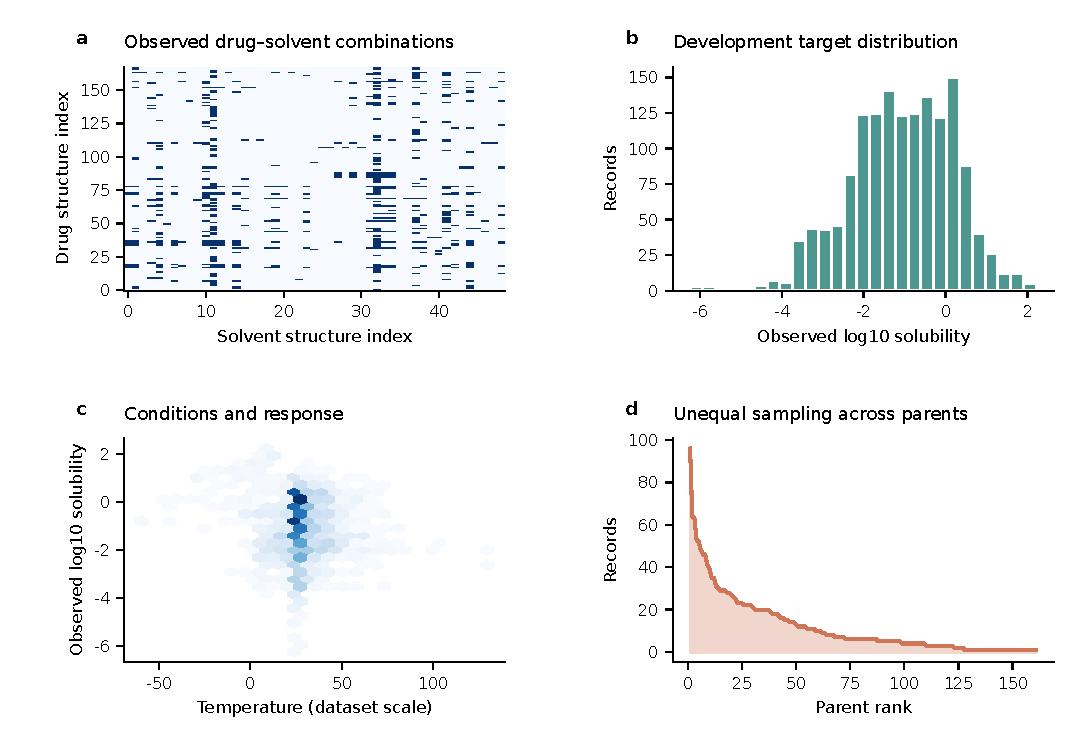
\includegraphics[width=\linewidth]{revision_v2/v2_data.pdf}
  \caption{数据覆盖、条件分布与采样频次。\textbf{a} 全量数据中观测到的完整药物与溶剂结构组合。\textbf{b,c} 开发集 1507 条记录的观测溶解度分布和温度与溶解度联合分布，颜色表示记录密度。\textbf{d} 全量数据的 161 个药物母体按观测数量排序。}
  \label{fig:v2-data-overview}
\end{figure}

\subsection{数据现象与设计假设}
有限的组合覆盖要求模型利用不同分子之间可比较的结构信息，因此后续比较基础描述符、丰富描述符与人工构造的药物--溶剂交互特征。母体频次不均意味着逐行平均误差更多反映高频母体的表现，因此将母体等权平均绝对误差作为主指标，并检验训练时采用母体加权的作用。存在温度变化的重复组合为组合内关联分析提供了观测基础，用于考察温度与溶解度在同一结构条件下如何共同变化。

\section{基于结构--温度分解的 SOLAR-H 溶解度预测模型}\label{sec:solar-method}

\subsection{设计动机}

在物理化学中，物质在溶剂中的溶解过程本质上受固液相平衡热力学所支配。根据经典 van 't Hoff 方程，摩尔溶解度随温度的变化由表观溶解焓 $\Delta H_{\mathrm{sol}}$ 调控：
\begin{equation}
\frac{\partial \ln S}{\partial (1/T)} = -\frac{\Delta H_{\mathrm{sol}}}{R},
\end{equation}
在有限的工业操作温区内，一阶局部泰勒近似表明对数溶解度与温度偏离基准值的位移量呈现近似线性依赖。更关键的是，$\Delta H_{\mathrm{sol}}$ 的大小直接由溶质分子与溶剂分子之间的溶剂化作用力与溶质晶格能的差额决定，具有强烈的化学结构特异性。

常规回归方法若直接将温度与高维分子特征并列输入黑盒模型，由于温度仅占单一维度且各组合测量温区不一，算法极易将温度变化与不同分子母体间的溶解度绝对水平发生混淆，导致学到的温度响应在未见母体上严重漂移。为此，本文设计了 SOLAR-H（Structured Orthogonal Linear \& Additive Regression -- Hybrid）模型，其核心思想是解耦预测目标：利用同一化学组合内部的温度变化正交估计局部温度响应斜率，继而在扣除温度项的基准目标上由树集成专门拟合分子结构基线。

\subsection{结构与温度分解}

设第 $i$ 条记录对应的药物--溶剂组合为 $c_i$。为刻画分子结构对温度敏感性的调控，提取药物与溶剂的 11 项基础物理化学描述符（分子量、MolLogP、TPSA、氢键供受体、芳香环数等），经训练折标准化后，构建包含原始值、Hadamard 元素乘积与绝对差值的 44 维结构特征向量 $z_c$。引入偏置项构建增广结构向量 $u_c = [1; z_c] \in \mathbb{R}^{45}$。

以当前训练集的温度中位数 $T_0$ 和四分位距 $s_T$ 对原始温度进行稳健标准化：
\begin{equation}
\tau_i = \frac{T_i - T_0}{s_T},
\end{equation}
SOLAR-H 模型将条件对数溶解度的预测值严密表示为结构基线与温度响应的加性组合：
\begin{equation}\label{eq:v2-solar}
\widehat y_i = b(z_c) + \gamma \cdot \tau_i \cdot \left( u_c^\top \beta \right),
\end{equation}
其中 $b(z_c)$ 表示在基准参考温度（$\tau_i = 0$，即 $T_i = T_0$）下的非线性化学结构基线，由 ExtraTrees 树集成进行拟合；$u_c^\top \beta$ 刻画组合 $c$ 对应的局部温度响应斜率，$\beta \in \mathbb{R}^{45}$ 为待学习的结构调制系数；$\gamma \in [0, 1]$ 为全局温度增益收缩超参数。

\subsection{组内去均值估计}

求解该模型面临的核心难点在于：未知的结构基线 $b(z_c)$ 具有高度复杂的非线性，若直接联合优化，参数 $\beta$ 极易受到分子间巨大溶解度绝对差异的强力干扰。

为解决这一问题，SOLAR-H 借鉴计量经济学面板数据中的固定效应消除技术。对于包含至少两个不同温度测量的训练组合 $c$，定义组内均值 $\bar y_c = \frac{1}{|c|}\sum_{i \in c} y_i$ 与 $\bar\tau_c = \frac{1}{|c|}\sum_{i \in c} \tau_i$。将式\eqref{eq:v2-solar}在组合内取均值并做差：
\begin{equation}
(y_i - \bar y_c) = \left[ b(z_c) - b(z_c) \right] + \gamma (u_c^\top \beta) (\tau_i - \bar\tau_c) + (\varepsilon_i - \bar\varepsilon_c).
\end{equation}
可以看到，复杂的未知非线性项 $b(z_c)$ 在组内差分中被完全数学消除。定义组内离差标签 $\Delta y_i = y_i - \bar y_c$，离差特征向量 $A_i = (\tau_i - \bar\tau_c) u_c^\top \in \mathbb{R}^{45}$。在基准增益 $\gamma = 1$ 下，参数 $\beta$ 的求解被严格转化为带母体加权与 $\ell_2$ 正则化的加权岭回归问题：
\begin{equation}
\widehat\beta = \arg\min_\beta \sum_{i: |\Delta\tau_i| > 0} w_i(q=1) (\Delta y_i - A_i \beta)^2 + \lambda \|\beta\|_2^2.
\end{equation}
令目标函数关于 $\beta$ 的梯度为零，可得严格的闭式解析解：
\begin{equation}
\widehat\beta = (A^\top W A + \lambda I)^{-1} A^\top W \Delta y,
\end{equation}
其中 $W$ 为由母体等权样本权重 $w_i(q=1)$（式\eqref{eq:v2-train-weight}）构成的对角矩阵，$\lambda$ 为岭正则化参数（固定为 1000 以确保高维数值求逆稳定性）。该估计式完全剥离了不同母体分子间的绝对溶解度差异，纯粹利用相同体系受温度驱动的热力学离差，从而获得了对物理温度效应的无偏估计。

\subsection{结构基线与联合求解}

在成功求得温度调制参数 $\widehat\beta$ 后，全量训练样本的温度贡献可被显式计算为 $\widehat\delta_i(\gamma) = \gamma \tau_i u_c^\top \widehat\beta$。随后，构造温度校正后的结构基线学习目标：
\begin{equation}
\widetilde y_i(\gamma) = y_i - \widehat\delta_i(\gamma).
\end{equation}
利用全部训练记录在校正目标 $\widetilde y_i$ 上训练母体等权 ExtraTrees 树集成，作为结构基线函数 $\widehat b(z_c)$。树模型配置 200 棵决策树，叶节点最小样本数为 1。

在内层三折嵌套验证中，联合网格搜索树深上限（8、16、不受限）及温度增益 $\gamma \in \{0, 0.1, 0.3, 1.0\}$，并以母体等权 MAE 为选择准则。选定最优参数后在外层训练集重新拟合，完成端到端联合求解。

\subsection{消融与自适应增益}

为深入探究 SOLAR-H 各核心模块对跨母体泛化性能的贡献，在外层 5 折交叉验证中实施了系统性的消融对比。保持相同的母体划分、测试集与随机种子，分别考察关闭母体加权（$q=0$）、关闭显式交互特征、完全关闭温度项（$\gamma=0$）以及强制满增益（$\gamma=1$）的影响。结果及配对 Bootstrap 95\% 置信区间如图\ref{fig:v2-solar-ablation}所示。

\begin{figure}[htbp]
\centering
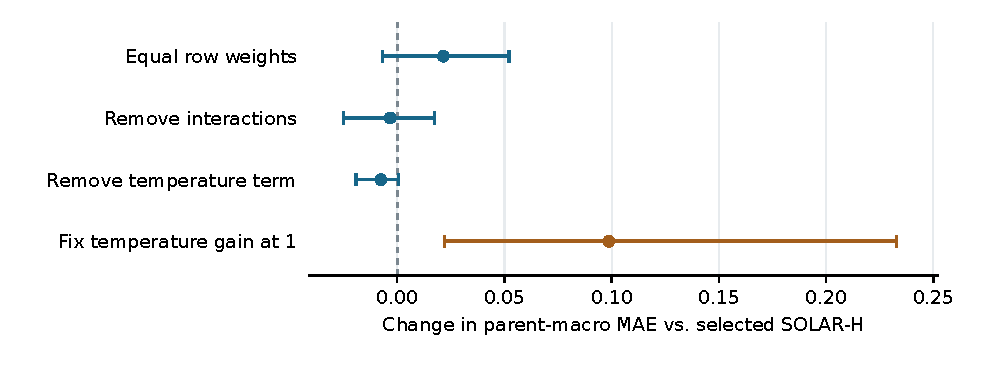
\includegraphics[width=\linewidth]{solar_ablation.pdf}
\caption{SOLAR-H 模型核心机制消融分析。点表示各消融配置相较基准自适应配置的母体等权 MAE 变化量（正值表示误差增加），误差棒表示 10,000 次母体配对 Bootstrap 抽样的 95\% 置信区间。}
\label{fig:v2-solar-ablation}
\end{figure}

消融实验揭示了模型深层的泛化机制。若关闭母体等权加权，SOLAR-H 在未见母体上的 MAE 恶化至 0.7380（上升 0.0216），表明样本重加权是克服高频母体支配、保障稀有母体基线拟合的关键。更为显著的是温度增益的外推效应：当强制设定满增益（$\gamma = 1.0$）时，未见母体 MAE 剧增至 0.8150（性能劣变 0.0987），证实小样本组合的狭窄温区极易受到测定噪声扰动，而内层嵌套自适应选择的收缩阻尼（$\gamma \in \{0, 0.1\}$）能有效抑制过度外推，在学习温度规律的同时确保了外推稳定性。

\subsection{本章小结}

本章构建了兼具热力学可解释性与统计严格性的 SOLAR-H 分解模型，通过组内固定效应消除了结构基线混杂，推导了加权岭回归闭式解，并通过内层嵌套验证确立了自适应增益机制。消融实验不仅验证了各组件的设计合理性，更在方法论层面指出了物理斜率向未知骨架迁移时必须配合自适应阻尼收缩的科学规律。
\section{模型设计与改进方法}
\label{sec:v2-methods}

\subsection{基础 ExtraTrees}
记第 $i$ 条记录的药物和溶剂为 $d_i$ 和 $s_i$，其温度为 $T_i$，标准化药物母体为 $g_i$。目标 $y_i$ 为记录中的对数溶解度。基础模型分别计算每种分子的 11 项描述符，涵盖分子量、MolLogP、拓扑极性表面积、氢键供受体数、可旋转键数、环数、芳香环数、重原子数、$sp^3$ 碳比例和形式电荷。药物与溶剂描述符加上温度形成 23 维输入。

ExtraTrees 在树节点中随机提出特征和切分点，并按平方误差下降幅度选择切分\cite{extratrees2006}。样本沿节点划分到叶，叶内目标均值给出该树的预测，集成预测取各树的平均。基础模型采用 200 棵树，按记录等权训练。候选配置改变树的深度上限、叶节点最小记录数和节点切分时的候选特征比例。这一基线用于评价仅以基础结构性质和温度为输入的树集成表现。

\subsection{丰富描述符与人工交互}
设 $D_i=\phi(d_i)$、$S_i=\phi(s_i)$。$\phi$ 按实验环境的 RDKit 描述符顺序计算 217 项属性。直接拼接的输入为 $[D_i;S_i;T_i]$，维数为 $2\times217+1=435$。为显式表示同名属性的共同取值与差异，构造
\begin{equation}
    x_i^{\mathrm{int}}=[D_i;S_i;T_i;D_i\odot S_i;|D_i-S_i|],
    \qquad \dim x_i^{\mathrm{int}}=4\times217+1=869.
\end{equation}
例如，MolLogP 的乘积和绝对差与两个原值共同输入树，允许节点分别按原始属性、共同取值或差异大小切分。第三种丰富表示在交互向量末尾加入标准化药物母体的 217 项描述符，共 1086 维。维数均指筛选前。丰富树在当前训练折中按列拟合中位数插补及零方差筛选，再将同一变换应用于相应验证数据。

\subsection{母体加权与叶节点预测}
对当前训练折 $\mathcal T$，令 $N_{\mathcal T}$ 为记录数，$G_{\mathcal T}$ 为母体数，$n_{g,\mathcal T}$ 为母体 $g$ 的记录数。为比较逐行等权与母体等权两种拟合，设置
\begin{equation}
    w_i(q)=
    \frac{n_{g_i,\mathcal T}^{-q}}
         {N_{\mathcal T}^{-1}\sum_{j\in\mathcal T} n_{g_j,\mathcal T}^{-q}},
    \qquad q\in\{0,1\}.
    \label{eq:v2-train-weight}
\end{equation}
$q=0$ 时 $w_i=1$。$q=1$ 时，分母为 $G_{\mathcal T}/N_{\mathcal T}$，因此每个母体的总权重均为 $N_{\mathcal T}/G_{\mathcal T}$。例如对全部开发记录拟合时，母体的总权重为 $1507/128\approx11.77$，同一母体的记录共享这份权重。

对节点中的记录集合 $L$，令节点拟合值为 $v$，平方误差为 $J_L(v)=\sum_{i\in L}w_i(q)(y_i-v)^2$。令 $\partial J_L/\partial v=0$，得到叶预测
\begin{equation}
    \widehat v_L=\frac{\sum_{i\in L}w_i(q)y_i}{\sum_{i\in L}w_i(q)}.
\end{equation}
对每个候选切分，比较父节点最小损失与两个子节点最小损失之和，选取降幅最大的切分。基础树的叶均值对应 $q=0$ 的情况。丰富描述符 ExtraTrees 固定 300 棵树，树深不设上限，叶节点至少含 2 条记录，节点候选特征比例为 0.7。三种丰富表示与两个 $q$ 值组成六项候选，采用母体等权平均绝对误差选择配置。节点拟合的加权平方误差与候选选择的绝对误差分别承担不同的计算任务。

\subsection{TabPFN 补充分支}
TabPFN v2 将当前训练折的特征与标签作为上下文，用固定的预训练权重对待预测记录推断其对数溶解度\cite{tabpfn2025}。令上下文为 $\mathcal C_{\mathcal T}=\{(x_i,y_i):i\in\mathcal T\}$，分支输出为预测分布的均值 $f_{\mathrm{PFN}}(x)=\mathbb E_{\theta}[Y\mid x,\mathcal C_{\mathcal T}]$。输入比较 23 维基础表示和 435 维丰富拼接表示，各自配置 2 或 4 个内部集成成员。两条预测分支均以原始对数溶解度标签为目标，树分支通过节点切分拟合本数据的非线性规律，TabPFN 通过训练折内的带标签上下文推断。

\subsection{分阶段配置选择与折外融合}
先在相同的内层母体划分上分别选择两条分支的配置，再按原始数据行对齐所选配置的折外预测。令 $p_i$、$t_i$ 分别为记录 $i$ 的 TabPFN 与 ExtraTrees 折外预测。采用 TabPFN 权重 $\alpha$ 时，预测为 $t_i+\alpha(p_i-t_i)$，残差可写成 $(y_i-t_i)-\alpha(p_i-t_i)$。这样可直接计算候选权重怎样改变树预测与观测值的距离。对内层折外集合中的 $G_{\rm in}$ 个母体，令 $I_g$ 为母体 $g$ 的记录集合，选权问题为
\begin{equation}
    \widehat\alpha
    =\arg\min_{\alpha\in\{0,0.25,0.5,0.75,1\}}
    \frac{1}{G_{\rm in}}\sum_g \frac{1}{|I_g|}\sum_{i\in I_g}
    \left|(y_i-t_i)-\alpha(p_i-t_i)\right|.
    \label{eq:v2-blend-selection}
\end{equation}
端点对应两条单分支。配置和权重选定后，在完整的外层训练部分重新拟合两条分支。验证记录的最终预测为
\begin{equation}
    \widehat y(x)=(1-\widehat\alpha)f_{\mathrm{ET}}(x)
                  +\widehat\alpha f_{\mathrm{PFN}}(x).
    \label{eq:v2-prediction-blend}
\end{equation}
部署模型在全开发集上重新执行三折配置与权重选择，随后使用全部 1507 条记录拟合。部署端固定使用交互表示、$q=1$ 的 ExtraTrees 和 23 维、2 成员的 TabPFN，分支权重分别为 0.75 和 0.25。外层评价中的权重由各折分别选定。

\subsection{替代设计与最终取舍}
早期探索比较过将结构基线与线性温度响应分开的 SOLAR-H。该模型用同一组合内的温度变化估计温度项，再在扣除温度项后的目标上拟合结构树。SOLAR-H 纳入同协议的历史对照。候选方案还包括先标准化再计算交互、限制每个母体的 TabPFN 上下文记录数，以及加入 CatBoost 等分支。部署方案保留原尺度交互和完整训练上下文，原尺度交互的选择参考同一三折划分下的筛查，最佳母体等权 MAE 为 0.6760，先标准化后计算交互的最佳结果为 0.6817。上下文与分支数量的比较见结果部分。

\section{实验设计与评价方法}
\label{sec:v2-experiments}

\subsection{数据划分与历史保留集用途}
数据划分将同一标准化药物母体的全部记录保留在同一部分。开发集包含 1507 条记录、128 个母体，历史保留集包含 397 条记录、33 个母体，两部分没有母体重叠。历史保留集曾用于早期模型的次级评价。本轮丰富特征与融合方案的结果来自开发集折外预测。

\subsection{嵌套选择、预处理与随机性}
采用固定的外层五折母体划分。每轮留出一折供评价，在其余四折内重新按母体分三折，分组打乱使用种子 2026。内层每次用两折拟合需要学习的数据变换和候选模型，在第三折生成预测。汇合三个内层验证折的预测后，分别选择分支配置，再按式\eqref{eq:v2-blend-selection}确定该外层折的融合权重。嵌套验证将配置选择置于外层训练部分，外层留出的母体为该流程提供误差估计\cite{varma2006}。

配置及权重由种子 2026 的内层预测确定，外层拟合采用 2026、17 和 42 三个种子，各种子使用相同划分与所选配置。多视角核回归的固定配置在同一折上复用确定性预测。特征填补、筛选、训练样本权重和 TabPFN 的带标签上下文均按当前训练折计算。

\subsection{对照模型与候选设置}
基础描述符 ExtraTrees 提供树集成基准，丰富描述符 ExtraTrees 和 TabPFN 提供与双分支直接对应的单模型对照，同时比较丰富树之间的融合及包含更多学习器的组合。表\ref{tab:v2-experiment-matrix}概括候选范围和比较目的。基础树与丰富树使用各自的树配置和搜索预算，二者的差值衡量整体建模流程的变化。丰富树的候选空间允许在同一表示下改变 $q$，也允许在固定 $q$ 时比较表示，两类候选在相同的内层数据上评分。主表的丰富树采用各折选出的配置，其得分同时反映表示与计权的选择。

\begin{table}[htbp]
  \centering\small
  \caption{主要比较对象及各外层训练部分的搜索范围。}
  \label{tab:v2-experiment-matrix}
  \begin{tabularx}{\linewidth}{@{}lX@{}}
    \toprule
    对象 & 配置与比较目的 \\
    \midrule
    基础 ExtraTrees & 12 项树配置，使用由基础描述符和温度组成的 23 维输入。 \\
    丰富描述符 ExtraTrees & 三种特征表示、两种计权方式，组成 6 项配置。 \\
    TabPFN v2 & 两种输入维度、两种分支内部成员数，组成 4 项配置。 \\
    其他单模型 & 丰富特征 CatBoost\cite{catboost2018}、多视角核回归和 TabM\cite{tabm2025}分别比较 6、10 和 2 项配置。 \\
    融合方案 & 基于所选分支预测搜索步长为 0.25 的非负权重，权重和为 1。对照包括不同分支数与组成。 \\
    \bottomrule
  \end{tabularx}
\end{table}

比较先从丰富表示与多视角组合展开，再加入 TabPFN。第二轮预先选定的主比较方案为 TabPFN 与丰富特征 ExtraTrees、CatBoost 的三分支组合。完整流程的选择继续参考这两轮的开发集外层结果，双分支方案在比较后进入后续诊断和部署。

\subsection{指标、汇总与配对不确定性}
对种子 $r$，将五个外层验证折拼接为覆盖 1507 条开发记录的折外预测，记 $e_i^{(r)}=\widehat y_i^{(r)}-y_i$，$I_g$ 为母体 $g$ 的记录集合，$G=128$，$N=\sum_g |I_g|=1507$。每个母体先计算其平均绝对误差，再对母体等权平均，
\begin{equation}
    A_g^{(r)}=\frac{1}{|I_g|}\sum_{i\in I_g}|e_i^{(r)}|,
    \qquad
    \mathrm{MAE}_{\mathrm{parent}}^{(r)}=\frac1G\sum_{g=1}^G A_g^{(r)}.
    \label{eq:v2-parent-mae}
\end{equation}
该量是主指标，衡量为每个母体赋予相同重要性时的预测误差。逐行 MAE 衡量每条记录的平均绝对偏差，均方根误差（RMSE）对大误差更敏感，
\begin{align}
    \mathrm{MAE}^{(r)} &= \frac1N\sum_{i=1}^N|e_i^{(r)}|
     =\sum_{g=1}^G\frac{|I_g|}{N}A_g^{(r)},\\
    \mathrm{RMSE}^{(r)} &= \sqrt{\frac1N\sum_{i=1}^N (e_i^{(r)})^2}.
\end{align}
上述三项指标以目标的对数尺度计量，越低表示误差越小。决定系数衡量相对于观测均值基准的平方误差变化，
\begin{equation}
    (R^2)^{(r)}=1-\frac{\sum_{i=1}^N(e_i^{(r)})^2}{\sum_{i=1}^N(y_i-\bar y)^2},
    \qquad \bar y=\frac1N\sum_{i=1}^N y_i.
\end{equation}
对于任一指标 $M$，取 $\overline M=\tfrac13\sum_r M^{(r)}$ 作为报告值。逐行分层误差沿用相同的逐行 MAE 公式，平均有符号误差使用该组内 $e_i^{(r)}$ 的算术平均。比较对照 $C$ 与融合方案 $F$ 时，MAE 的相对降幅为 $100\%\times(\overline M_C-\overline M_F)/\overline M_C$。

母体配对比较在同一母体、同一种子上计算两种方法的差值，
\begin{equation}
    d_g=\frac13\sum_r\left(A_{g,F}^{(r)}-A_{g,C}^{(r)}\right),
    \qquad
    \Delta=\frac1G\sum_{g=1}^G d_g.
    \label{eq:v2-paired-delta}
\end{equation}
负值表示融合方案误差较低。以种子 2026 有放回地从 128 个母体索引中抽取 128 个，每次计算对应 $d_g$ 的均值，共重复 10000 次，取其第 2.5 与第 97.5 百分位数作为 95\% 配对 bootstrap 区间。重采样使用已保存的折外预测，区间反映既定方案下母体误差差值的抽样变动。

\subsection{运行环境与复现材料}
丰富树与融合实验采用 Python 3.12、RDKit 2026.9.2、scikit-learn 1.9.1、TabPFN 6.4.1 和 PyTorch 2.15.0，TabPFN v2 在 Apple Silicon 的 MPS 设备上运行。项目保留原始行号到母体与验证折的映射、候选配置和折级选权记录、按行与种子保存的预测、部署模型及其配置元数据。

\section{预测结果、误差与稳健性}\label{sec:prediction_results}

\subsection{总体性能}
基础 ExtraTrees、丰富特征 ExtraTrees 与双分支融合的母体等权 MAE 依次为 0.7469、0.6831 和 0.6668。融合流程在所比较的开发集方案中取得最低观测误差，逐行 MAE 为 0.6510，RMSE 为 0.8842，$R^2$ 为 0.5234。表\ref{tab:v2_main_metrics} 以基础树和丰富特征树为比较起点，同时列出 TabPFN 单分支和两种包含更多候选分支的融合方案，便于评价表示扩展与融合的增量表现。

\begin{table}[htbp]
\centering
\small
\caption{开发集母体分组外层验证结果。每个种子先在合并的五折预测上计算四项指标，再对三个种子取平均。前三项误差使用对数溶解度尺度，$R^2$ 无量纲。}
\label{tab:v2_main_metrics}
\begin{tabular}{lrrrr}
\toprule
模型流程 & 母体等权 MAE & 逐行 MAE & RMSE & $R^2$ \\
\midrule
基础描述符 ExtraTrees & 0.7469 & 0.7491 & 0.9730 & 0.4229 \\
丰富特征 ExtraTrees & 0.6831 & 0.6720 & 0.8981 & 0.5083 \\
TabPFN 单分支 & 0.6827 & 0.6698 & 0.9117 & 0.4933 \\
ExtraTrees 与 TabPFN 融合 & \textbf{0.6668} & \textbf{0.6510} & \textbf{0.8842} & \textbf{0.5234} \\
TabPFN 与双树融合 & 0.6729 & 0.6631 & 0.8882 & 0.5191 \\
五候选分支融合 & 0.6767 & 0.6568 & 0.8899 & 0.5172 \\
\bottomrule
\end{tabular}
\end{table}

\subsection{改进来源与融合增量}
丰富特征树的母体等权 MAE 较基础树降低 0.0638（8.54\%）。以丰富特征树减基础树计算差值，95\% 母体配对区间为 $[-0.1219,-0.0082]$。这项差异对应描述符、模型配置及训练策略共同变化后的整体表现。为进一步区分设计因素，表\ref{tab:v2_tree_pilot} 报告此前三折分组筛查的四个 ExtraTrees 对照。固定 300 棵树、无深度上限、叶节点最小样本数 2、特征采样比例 0.7 以及相同划分后，增加交互特征使 $q=0$ 和 $q=1$ 时的母体等权 MAE 分别下降 0.0127 和 0.0093。逐行等权切换为母体等权训练时，两种表示下的观察降幅分别为 0.0258 和 0.0225。这些比较说明两项设计在该轮筛查中的方向一致。其数值按单一种子和三折划分计算，适合用于理解设计选择。

\begin{table}[htbp]
\centering
\small
\caption{丰富特征 ExtraTrees 的三折开发集筛查。各格为母体等权 MAE，使用同一分组划分、种子 2026 及树参数。}
\label{tab:v2_tree_pilot}
\begin{tabular}{lrr}
\toprule
结构表示 & 逐行等权（$q=0$） & 母体等权（$q=1$） \\
\midrule
丰富描述符拼接 & 0.7112 & 0.6853 \\
拼接、逐元素乘积与绝对差 & 0.6985 & 0.6760 \\
\bottomrule
\end{tabular}
\end{table}

在对齐的外层折外预测中，融合较丰富特征 ExtraTrees 和 TabPFN 的母体等权 MAE 分别减少 0.0163 和 0.0159，相对降幅为 2.39\% 和 2.32\%。对应的 95\% 配对区间分别为 $[-0.0370,0.0001]$ 和 $[-0.0478,0.0178]$（融合减对照）。两个区间都覆盖零，增量收益的稳定性有待锁定方案后的新数据评价。逐条有符号残差的 Pearson 相关系数为 0.909，说明两分支的偏差方向往往相近，融合的价值应结合具体母体的改善与退化判断。

\subsection{母体与目标区间误差}
融合模型的逐母体 MAE 中位数为 0.544，第 90 百分位数为 1.355，最大值为 2.670。与丰富特征树相比，128 个母体中有 61 个误差下降、41 个上升，26 个持平。26 个持平母体位于将 TabPFN 权重设为零的外层折上。与 TabPFN 相比，65 个母体改善，63 个退化。均值变化因此掩盖了母体间差异。

\begin{table}[htbp]
\centering
\small
\caption{融合流程按实测溶解度划分的开发集外层折外误差。记录数和母体数按区间内的唯一观测和母体计数，同一母体可出现在多个区间。各指标在区间内对记录和三个种子等权平均。有符号误差定义为预测值减实测值，正值表示高估。}
\label{tab:v2_target_band_errors}
\begin{tabular}{lrrrr}
\toprule
实测对数溶解度 & 记录数 & 母体数 & MAE & 平均有符号误差 \\
\midrule
$y\leqslant-4$ & 23 & 8 & 2.251 & $+2.250$ \\
$-4<y\leqslant-2$ & 321 & 56 & 0.874 & $+0.784$ \\
$-2<y\leqslant0$ & 824 & 110 & 0.465 & $-0.120$ \\
$y>0$ & 339 & 43 & 0.782 & $-0.772$ \\
\bottomrule
\end{tabular}
\end{table}

误差随实测溶解度区间而变化（表\ref{tab:v2_target_band_errors}）。低值区的 23 条记录平均被高估约 2.25 个对数单位，$y>0$ 的记录则呈低估。以跨种子的平均绝对误差选出误差最大的记录为例，蔗糖在氯仿中、温度原始数值为 25 时，实测对数溶解度为 $-6.234$，三个种子的平均预测为 $-2.536$。对应外层训练部分含 98 条氯仿记录，温度范围为 $[-29.2,55.05]$。即使溶剂和温度落在训练数据覆盖内，目标值极低的未见母体仍可能被明显高估。

\subsection{权重、随机种子与上下文设置}
五个外层折通过内层验证得到的 TabPFN 权重依次为 0.25、0.25、0、0.25、0.50，反映了训练样本变化下的选权差异。在已保存的单分支折外预测上，把 TabPFN 权重固定为 0.25、0.50 或 0.75，得到的母体等权 MAE 分别为 0.6734、0.6708、0.6732（图\ref{fig:v2_prediction_diagnostics}b）。该事后曲线刻画固定权重的敏感程度。主结果 0.6668 对应各折独立地在内层选择权重的验证流程。按种子 17、42、2026 分别汇总，该流程的母体等权 MAE 为 0.6635、0.6679、0.6690，范围宽度为 0.0056；这三个结果来自同一外层划分。

另一项三折筛查固定 TabPFN 的 23 维基础输入及四成员配置，检查训练折内对每个母体设置上下文记录上限的影响。完整上下文的母体等权 MAE 为 0.7252，每个母体最多保留 32 条时为 0.7148，限制至 16 条和 8 条时分别增至 0.7466 和 0.7807。温和裁剪在该筛查中有小幅收益，进一步收紧则伴随误差上升。这些结果描述上下文规模的取舍，正式双分支流程继续使用完整训练折上下文。

\begin{figure}[htbp]
\centering
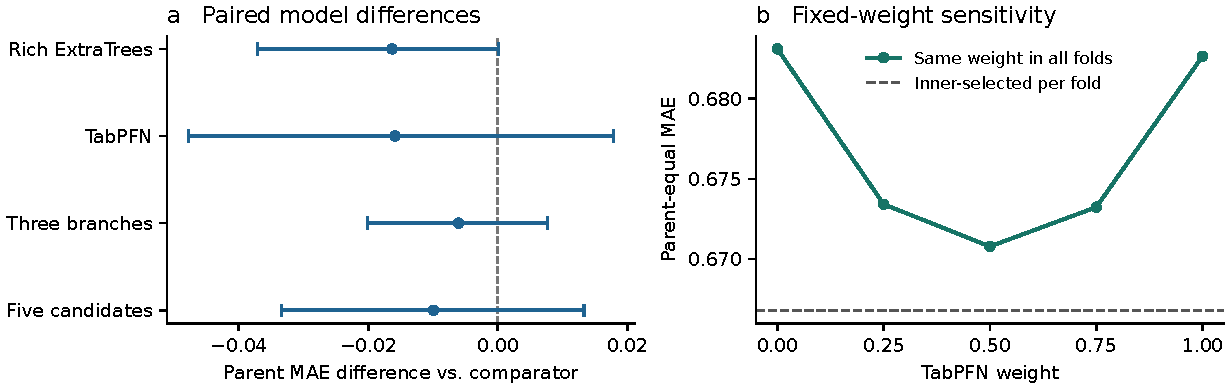
\includegraphics[width=\linewidth]{prediction_diagnostics.pdf}
\caption{融合流程的配对差值及固定权重灵敏度。\textbf{a} 差值为双分支融合减对照的母体等权 MAE，负值表示融合误差较小。区间对 128 个母体配对重采样 10000 次，保存的折外预测保持固定。\textbf{b} 将同一权重用于各外层折的两支折外预测，图中虚线为内层按折选权流程的观测误差。两幅图均基于 1507 条开发记录。}
\label{fig:v2_prediction_diagnostics}
\end{figure}

\subsection{性能与复杂度取舍}
加入 CatBoost 的三候选分支方案和允许五个分支参与选权的方案，母体等权 MAE 分别为 0.6729 与 0.6767。相对这两种方案，双分支的观测差值分别为 $-0.0061$ 和 $-0.0099$，母体配对区间为 $[-0.0201,0.0076]$ 和 $[-0.0334,0.0133]$（图\ref{fig:v2_prediction_diagnostics}a）。五候选方案在各外层折实际启用三个非零分支，表明扩大候选集合也会改变权重选择和配置复杂度。双分支在本次比较中的平均误差较低，部署时需管理的模型也较少，因此被选为应用方案。

\section{模型可解释性与温度作用分析}

\subsection{分析目标}

在药物研发与工艺设计中，高精度的机器学习模型若缺乏透明的决策逻辑，将难以赢得药物化学家的信任，更无法为分子修饰或工艺改进提供指导。本章聚焦两项核心机理问题：深入解析 ExtraTrees--TabPFN 模型的特征归因与 TabPFN 的局部校正路径，并系统探究温度与溶解度的物理因果关联，检验模型温度响应的真实性。

\subsection{SOLAR-H 结构贡献}

SOLAR-H 模型在数学架构上天然具备白盒透明度。根据式\eqref{eq:v2-solar}，模型输出严格由两部分线性叠加而成：
\begin{equation}
\widehat y_i = \underbrace{\widehat b(z_c)}_{\text{结构常数项}} + \underbrace{\gamma \cdot \tau_i \cdot \left( u_c^\top \widehat\beta \right)}_{\text{结构调制的温度响应项}}.
\end{equation}
对于任意固定的药物--溶剂组合 $c$，模型对温度的响应导数恒定为 $\frac{\partial \widehat y}{\partial T} = \frac{\gamma u_c^\top \widehat\beta}{s_T}$。在全量开发集部署配置中，由于内层嵌套验证自动选取了高阻尼增益 $\gamma = 0$，模型自适应退化为结构基线预测，有效杜绝了因温度噪声在未见母体上的外推漂移。当在训练折选用非零增益时，参数 $\widehat\beta$ 显式反映了分子量差异、极性失配对吸热溶解斜率的调节方向。

\subsection{特征归因}\label{sec:deployment-explanations}

对于非线性的 ExtraTrees--TabPFN 工业部署模型，本研究结合博弈论 Shapley 值与局部分支贡献展开双重归因分析。

\subsubsection{TreeSHAP 全局特征组归因分析}
对于 ExtraTrees 树分支，采用基于树路径依赖的 TreeSHAP 算法\cite{treeshap2020}。在 128 个开发母体中均衡抽取覆盖全量化学空间的 227 条解释样本。TreeSHAP 算法在浮点精度级别满足局部准确性公理（重构预测偏差低于 $1.3\times10^{-13}$），基线参考期望值（背景预测值）为 $-1.1632$。

将模型保留的 665 个高维特征按照化学物理属性归集为四大功能组：药物描述符、溶剂描述符、温度特征以及显式分子间交互特征。各组的有符号归因绝对值在 128 个母体维度等权平均后的结果如图~\ref{fig:deployment-explanations}A 所示。

\begin{figure}[htbp]
\centering
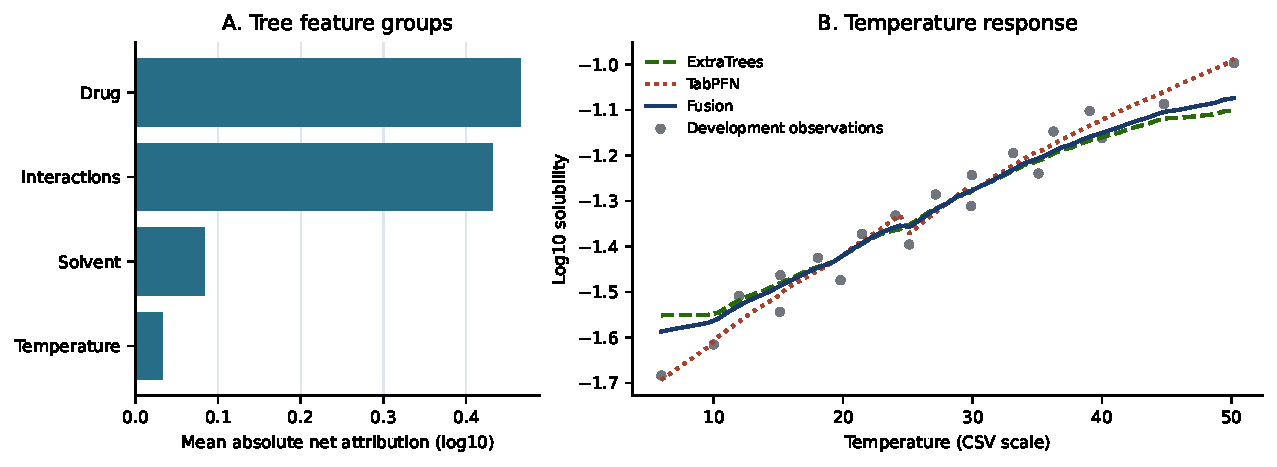
\includegraphics[width=\linewidth]{deployment_explanations.pdf}
\caption{部署模型的特征归因与温度动态响应分析。\textbf{A} 四大功能特征组的母体等权绝对净归因对比；\textbf{B} 洛伐他汀--乙酸丁酯组合在观测温区内的预测曲线（散点为真实测量点，实线为融合预测，虚线为各单分支响应）。}
\label{fig:deployment-explanations}
\end{figure}

归因结果具有明确的化学含义。药物描述符（平均绝对归因 0.466）与显式交互特征（0.432）的归因值最高。这与溶液物理化学一致：药物分子结构庞大复杂（分子量通常在 200--800 之间），其固态晶格能与固相内聚强度是溶解需要克服的晶格能项；而溶质与溶剂之间的显式交互（极性匹配与氢键配对）直接决定了溶剂化放热能否克服晶格能。相比之下，溶剂描述符（0.084）与温度特征（0.033）起精细微调作用。由于溶剂库相对有限（49 种常见工业溶剂）且结构较为规整，其单独贡献相对集中，更多作为条件扰动在宏观结构基线上进行局部调节。

\subsubsection{TabPFN 的局部分支动态校准机理}
为探究 TabPFN 如何与 ExtraTrees 协同工作，表~\ref{tab:deployment-examples}选取了部署模型中 TabPFN 修正量 $\Delta_{\mathrm{PFN}} = 0.25 (f_{\mathrm{PFN}} - f_{\mathrm{ET}})$ 呈现极大与极小极端调节的两条真实案例。

\begin{table}[htbp]
\centering\small
\setlength{\tabcolsep}{4pt}
\caption{部署模型中 TabPFN 对 ExtraTrees 分支进行双向微调校准的典型案例分析（两例均以丙酮为溶剂）。}
\label{tab:deployment-examples}
\begin{tabular}{lrrrrrr}
\toprule
候选药物（数据索引） & 温度 ($^\circ\text{C}$) & 实测值 & ExtraTrees & TabPFN & 融合预测 & 修正量 $\Delta_{\mathrm{PFN}}$ \\
\midrule
赤藓糖醇（样本行 23） & 13.2 & $-2.692$ & $-2.495$ & $-2.716$ & $-2.551$ & $-0.055$（下调） \\
对羟基苯甘氨酸 Dane 盐（样本行 3） & 70.2 & $-1.843$ & $-1.927$ & $-1.847$ & $-1.907$ & $+0.020$（上调） \\
\bottomrule
\end{tabular}
\end{table}

两项案例生动展现了异质集成的自适应校正机制。在赤藓糖醇案例中，ExtraTrees 受到常温多羟基化合物统计均值的牵引，对数预测为 $-2.495$（显著高估实测值 $-2.692$）。TabPFN 基于连续注意力空间识别出其高极性小分子在低极性溶剂中的不溶性特征，给出更低的 $-2.716$ 预测，驱动融合模型向下校正至 $-2.551$，大幅缩减了绝对误差。在 Dane 盐案例中，ExtraTrees 预测偏保守（$-1.927$），而 TabPFN 准确捕捉到 $70.2^\circ\text{C}$ 高温下的热力学促溶效应，给出 $-1.847$ 预测，驱动融合模型向上微调至 $-1.907$，逼近实测值 $-1.843$。上述对比确证了 TabPFN 依托其丰富的先验流形表征，在不同化学空间动态实施方向完全不同的有效纠偏。

\subsection{动态温度响应}

为检验模型在连续温度变化下的物理合理性，固定洛伐他汀--乙酸丁酯体系（该体系在开发集中包含 20 个密集的温度实测点，温区跨度为 $[5.95^\circ\text{C}, 50.2^\circ\text{C}]$），对输入温度进行等距致密扫描（图~\ref{fig:deployment-explanations}B）。

扫描曲线清晰地表明：ExtraTrees 表现出阶梯状分段非线性，反映了轴切分树模型的典型离散特性；而融合模型展现出平滑、单调向上的连续响应曲线，对数溶解度预测值从 $5.95^\circ\text{C}$ 下的 $-1.587$ 稳步递增至 $50.2^\circ\text{C}$ 下的 $-1.074$；预测曲线紧密穿过真实实验观测散点簇的中枢，高度符合大多数固液溶质吸热溶解的宏观物理热力学规律，证实模型学到了物理一致的温变行为。
\section{温度关联分析与因果识别边界}\label{sec:temperature-association}

\subsection{温度干预问题与假设图}
对给定的完整药物形式和溶剂组成，因果问题是按同一实验协议将体系从温度 $t_0$ 调至 $t_1$ 并达到相应平衡时，对数溶解度会改变多少。用 $D$ 和 $S$ 表示观测到的药物与溶剂，$T$ 和 $Y$ 表示记录温度和对数溶解度，$U$ 表示未记录的实验条件。以下有向关系给出识别所依赖的假设\cite{pearl2009}：
\begin{equation}
(D,S)\longrightarrow T,\qquad (D,S)\longrightarrow Y,\qquad
U\longrightarrow T,\qquad U\longrightarrow Y,\qquad T\longrightarrow Y.
\end{equation}
药物与溶剂可能同时影响温度选择和溶解度，实验来源或协议也可能同时影响二者。$T\to Y$ 表示拟考察的因果路径。温度字段沿用 CSV 原始数值尺度，以下斜率以每一原始温度单位对应的对数溶解度变化表示。

\subsection{总体关联与组合内关联}
在开发集中，以规范化的完整药物与完整溶剂结构定义组合，保留每个组合内至少两个不同温度的记录。得到 157 个组合、73 个药物母体和 1118 条记录。各组合内温度跨度为 5.00 至 65.15 个原始单位，中位数为 27.10。在相同的 1118 条记录上，先按逐行线性回归估计总体斜率，再以组合固定效应估计共同的组内斜率。令 $c$ 表示组合，$i$ 表示组合内记录，则
\begin{align}
Y_{ic}&=\alpha_c+\beta T_{ic}+\varepsilon_{ic},\\
\hat\beta&=\frac{\sum_c\sum_i(T_{ic}-\bar T_c)(Y_{ic}-\bar Y_c)}
{\sum_c\sum_i(T_{ic}-\bar T_c)^2}.
\end{align}
组合内去均值可消去 $\alpha_c$，使斜率由同一组合内的温度和溶解度共同变化决定。若各组合的斜率不同，共同斜率相当于按组合内温度离差平方和加权，温区较宽或记录较多的组合可占较大权重。

\subsection{估计结果与不确定性}
同一子集上，总体斜率点估计为负，组内点估计为正（表~\ref{tab:temperature-association}）。总体区间覆盖零。在相同药物与溶剂的记录之间比较时，较高温度与较高溶解度相联系。按母体进行 2000 次有放回重采样，各次均保留被抽中母体的全部组合和记录，得到组内斜率的 95\% 百分位区间 $[0.01236,0.01902]$。逐一删去母体后的斜率范围为 $[0.01424,0.01599]$，各次估计保持正向。

\begin{table}[htbp]
\centering\small
\caption{相同 1118 条记录上的总体和组合内斜率。单位为每一 CSV 原始温度单位对应的对数溶解度变化，95\% 区间采用母体聚类稳健标准误。}
\label{tab:temperature-association}
\begin{tabular}{lrr}
\toprule
估计口径 & 斜率 & 95\% 区间\\
\midrule
逐行总体回归 & $-0.00746$ & $[-0.02614,\phantom{-}0.01123]$\\
组合内固定效应 & $\phantom{-}0.01538$ & $[\phantom{-}0.01198,\phantom{-}0.01878]$\\
\bottomrule
\end{tabular}
\end{table}

\subsection{未测混杂与识别条件}
固定效应控制组合内稳定的差异，实验来源、协议等若随温度记录变化，仍可形成温度与溶解度的共同影响。pH 和晶型的角色取决于测量顺序及干预条件。若它们随温度变化，固定或调整它们会改变所对应的因果问题。在去组均值线性模型中，进一步衡量未测变量对斜率点估计的影响\cite{sensitivity2020}。记 $r_T$ 为该变量与温度在控制组合后的偏 $R^2$，$r_Y$ 为该变量与溶解度在控制温度与组合后的偏 $R^2$。在设定 $r_T=r_Y$ 且偏倚方向使观测斜率增大的情形下，两者约需同为 0.54 才能使调整后的斜率降为零。该数值用普通最小二乘的遗漏变量偏倚恒等式计算，刻画点估计对假设混杂强度的敏感性。

要将组内关联解释为干预效应，需核实温标，在可比协议下明确温度与平衡状态，并在有共同温度支持的组合内测量或控制先于干预的混杂因素。当前估计描述实测组合内的关联，后续可通过受控温度实验检验这一关系。

\section{系统实现与应用验证}\label{sec:v2-application}

\subsection{架构与部署配置}

系统采用静态网页与 FastAPI 服务。用户从药物和溶剂目录中选择结构，输入温度并指定模型。服务将目录标识转换为完整 SMILES，核验模型文件的 SHA-256，加载相应预处理器与模型。默认模型版本为 \texttt{a3536da9c926}（文件散列前 12 位），使用全部开发记录拟合，树分支采用 869 维交互表示，预处理后输入 665 列，TabPFN 读取保存的训练上下文。系统按 ExtraTrees 权重 0.75、TabPFN 权重 0.25 计算对数溶解度，再按 CSV 的浓度字段对预测作 $10^{\widehat y}$ 反变换。图\ref{fig:v2-app-flow}给出服务处理链。

\begin{figure}[htbp]
\centering\small
\fbox{\begin{minipage}{0.91\linewidth}
\centering
分子目录与温度输入 $\longrightarrow$ 结构解析与描述符计算\\[4pt]
$\longrightarrow$ ExtraTrees 与 TabPFN 分支预测 $\longrightarrow$ 加权求和\\[4pt]
$\longrightarrow$ 预测值、分支输出与开发集数据覆盖
\end{minipage}}
\caption{默认模型从输入选择到结果展示的处理顺序。数据覆盖单独查询开发集，模型评价页另读取外层折外指标。}
\label{fig:v2-app-flow}
\end{figure}

\subsection{洛伐他汀在丙酮中的预测案例}

以洛伐他汀、丙酮和原始尺度温度 25 为例，界面返回对数溶解度 $-0.7270$，按 CSV 单位显示反变换浓度 $0.1875\,\mathrm{mol/L}$。ExtraTrees 预测约为 $-0.7221$，TabPFN 预测约为 $-0.7415$。用户可在同一药物和溶剂条件下查看温度曲线，或与基础 ExtraTrees 的预测作逐点比较。数据支持区域显示该组合有 20 条开发观测，温度覆盖为 5.5 至 49.5。这些观测构成部署模型的数据背景。系统另提供 CSV 批量入口用于比较候选条件。

\begin{figure}[H]
\centering
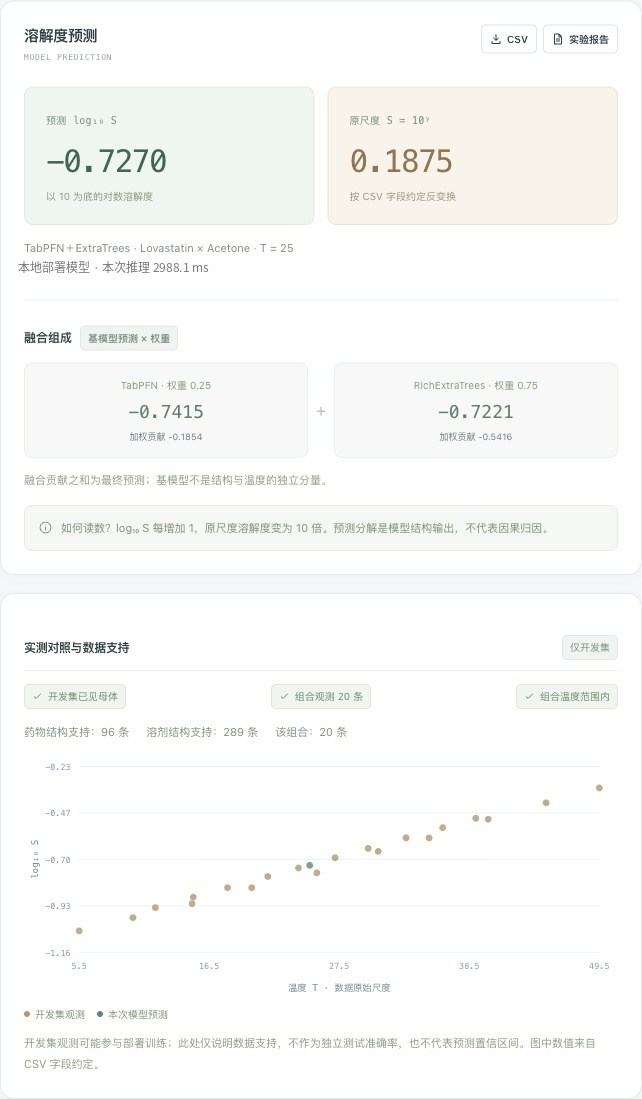
\includegraphics[width=\linewidth,height=0.51\textheight,keepaspectratio]{app_prediction.jpg}
\caption{应用中的洛伐他汀--丙酮单点预测。上部显示对数预测及反变换浓度，中部显示分支预测和权重，下部显示同一组合的开发集观测。温度采用 CSV 数值尺度。}
\label{fig:v2-app-example}
\end{figure}

\subsection{一致性、输入处理与运行表现}

通过进程内 HTTP 测试核对实际接口与离线模型。单点接口与离线调用在相同输入下达到 $10^{-8}$ 的对数预测绝对差容差，两个分支的加权贡献之和也与接口输出一致。对照接口对两个模型使用相同的 61 个温度点，并返回共同的 128 个母体的折外误差。该条件的 61 点曲线在温度 25 处与单点调用的绝对差为 $4.92\times10^{-7}$。批量接口允许 1--100 行，含无效温度的一行由该行返回错误，其余有效样本照常输出。复现脚本与核对结果保存在报告目录。
在 Apple Silicon 的 MPS 环境中，同一条件进行一次预热后，连续五次单行推理的服务端计时中位数为 2.32 秒，范围为 2.25 至 2.32 秒。该计时记录的是服务端模型计算，适用于此次设备和请求规模。

\section{综合讨论与研究局限}

\subsection{表示设计与融合增量}

对 RQ1，主要的误差下降出现在从基础 ExtraTrees 改为丰富特征树的阶段，说明在此任务中优先改进树分支具有价值。三折筛查在固定树参数和分组的条件下提供了更具体的证据：加入显式交互和采用母体加权时，观察到的误差均向下变化。五折评价中的丰富树会逐折选择特征和加权配置，因此整体改善包括这些选择的共同作用。

对 RQ2，TabPFN 进一步降低了平均误差，但融合收益小于从基础树到丰富树的变化。不同外层折选出的权重及母体间的误差差异说明，补充分支的价值取决于样本组成。复杂度较低的ExtraTrees 单模型适合作为快速回归基准，当前双分支适合需要同时查看两种学习器预测的条件筛选。模型流程经过两轮开发比较后确定，锁定方案后在独立来源数据上验证，才能评价这一增量能否重复。

\subsection{预测依据与推广范围}

对 RQ3，特征归因和温度扫描说明了部署模型如何利用结构与条件信息。组合内实测分析提供另一种证据，即同一完整药物--溶剂配对内部，温度与测量值如何共同变化。两类证据分别有助于检查模型行为和理解数据构成。记录缺少测量规程和样品状态等元数据，温度的干预效应需要有可比条件的测量才能估计。

母体分组验证直接对应已观测数据来源中的未见母体预测。推广到未见骨架时可采用骨架分组，推广到未见溶剂时需单独留出溶剂，超出观测温区的可靠性应通过该温区的实测记录核验。低溶解度记录的系统性高估会影响筛选排序，宜在独立评价中优先检查这一目标区间，并用独立于最终评价的样本拟合和验证校准方案。

\section{结论}

\subsection{主要发现}

本研究以药物母体为评价单位，比较了描述符扩展和异质模型融合对条件溶解度预测的影响。基础 ExtraTrees、丰富特征 ExtraTrees 和双分支融合在开发集的母体等权 MAE 分别为 0.7469、0.6831 和 0.6668。主要改善来自树分支整体设计的变化，融合在当前比较中提供了较小的增量，且配对区间反映出该增量仍有波动。误差分析将低溶解度端确定为优先核验的场景。

\subsection{方法与应用交付}

交付包括从结构描述符计算、训练折内选择到母体折外评价的建模流程，以及部署双分支模型的交互应用。系统可在指定条件下给出预测、分支贡献、温度曲线和开发集覆盖信息。后续可将固定模型用于独立来源数据，先检查低溶解度端和新化学骨架上的偏差，再评估校准方法能否改善筛选表现。

\FloatBarrier
\newcommand{\BIBdecl}{\fontsize{10}{13}\selectfont\setlength{\itemsep}{0.1em}\setlength{\parsep}{0pt}}
\bibliographystyle{IEEEtran}
\bibliography{references}
\end{document}
